\documentclass[10pt,a4paper]{article}
\usepackage[T1]{fontenc}
\usepackage[utf8]{inputenc}
\usepackage{lmodern,microtype}
\usepackage[margin=17mm,top=17mm,bottom=18mm,headheight=14pt]{geometry}
\usepackage{amsmath,amssymb,booktabs,tabularx,array,multicol,xcolor}
\usepackage{graphicx,tikz,pgfplots,tcolorbox,enumitem,fancyhdr,titlesec,caption}
\usetikzlibrary{arrows.meta,positioning,shapes.geometric}
\pgfplotsset{compat=1.18}
\definecolor{navy}{HTML}{17334D}
\definecolor{teal}{HTML}{087F8C}
\definecolor{muted}{HTML}{596977}
\definecolor{pale}{HTML}{EDF5F6}
\definecolor{orange}{HTML}{C36B32}
\usepackage[colorlinks=true,urlcolor=teal,linkcolor=navy]{hyperref}
\hypersetup{pdftitle={BioPrint: Adaptive Behavioral Verification},pdfauthor={BioPrint},pdfsubject={Final six-page research and implementation report}}
\pagestyle{fancy}\fancyhf{}
\fancyhead[L]{\small\sffamily\bfseries\color{navy}BIOPRINT\quad\normalfont\small Research \& implementation}
\fancyhead[R]{\small\sffamily\color{muted}FINAL REPORT}
\fancyfoot[L]{\scriptsize\color{muted}Dataset evidence \;\textbullet\; Synthetic policy evaluation \;\textbullet\; Working prototype}
\fancyfoot[R]{\small\thepage\,/\,6}
\renewcommand{\headrulewidth}{0.3pt}
\titleformat{\section}{\large\sffamily\bfseries\color{navy}}{\thesection}{0.6em}{}
\titleformat{\subsection}{\normalsize\sffamily\bfseries\color{teal}}{\thesubsection}{0.5em}{}
\titlespacing*{\section}{0pt}{10pt}{6pt}
\titlespacing*{\subsection}{0pt}{8pt}{4pt}
\setlength{\parindent}{0pt}\setlength{\parskip}{4pt}
\setlength{\tabcolsep}{4pt}\renewcommand{\arraystretch}{1.15}
\setlist{nosep,leftmargin=1.4em}
\captionsetup{font=small,labelfont=bf,skip=4pt,hypcap=false}
\newcommand{\note}[1]{\begin{tcolorbox}[colback=pale,colframe=teal,boxrule=0pt,leftrule=2pt,arc=0pt,left=7pt,right=7pt,top=5pt,bottom=5pt]#1\end{tcolorbox}}
\newcommand{\triple}[3]{#1 / #2 / #3}
\newcommand{\smalltable}{\fontsize{8.5}{10.4}\selectfont}
\begin{document}
\thispagestyle{fancy}
{\sffamily\color{teal}\small ACCOUNT-HOLDER VERIFICATION\par}
{\sffamily\bfseries\color{navy}\fontsize{28}{32}\selectfont BioPrint\par}
{\sffamily\color{navy}\Large Recognize the behavior behind the password\par}
{\large An evidence-led design for adaptive typing--pointer verification\par}
\vspace{4pt}
\note{\textbf{Abstract.} BioPrint adds behavioral verification to password login: typing provides the first identity signal, device fingerprinting supplies context, and uncertain attempts receive a pointer or keypad challenge. We develop this design through public-dataset comparisons, paired-modality studies and controlled synthetic login experiments. A trained pointer encoder reduces synthetic false acceptance from \textbf{14/90 to 9/90}, with a corresponding increase in genuine rejection from \textbf{13/60 to 19/60}. Typing experiments show improved separation with richer enrollment and nonlinear models. The resulting system combines inexpensive initial checks with targeted additional evidence, while preserving explicit model compatibility and a reproducible demonstration of both successes and failures.}

\section{Introduction: verifying the operator, not only the secret}
A correct password proves knowledge of a secret; it does not distinguish its owner from another person who has obtained it. Device recognition addresses a different question: whether the browser and computer are familiar. An impostor on the owner's laptop may have a perfect device match, while the legitimate owner may arrive on a new phone. BioPrint treats these as complementary signals rather than allowing a familiar device to substitute for behavioral identity.

Behavioral biometrics analyzes how a person interacts: the durations and overlap of keystrokes, movement toward targets, and the timing of visual search and selection. Commercial systems such as BioCatch use physical and cognitive behavior in fraud detection [2]. The National Institute of Standards and Technology (NIST) distinguishes such fraud indicators from authentication factors [1]. BioPrint applies this principle to an inspectable login prototype; it is an additional account-risk layer, not a claimed replacement for cryptographic authentication.

\subsection{The design argument}
The goal is to reduce impostor access without challenging every genuine login. Typing is already present in password entry, so it is the natural first behavioral measurement. Pointer motion offers a different observation when typing is inconclusive. Device fingerprinting helps decide when stronger evidence is needed, while bot checks identify scripted or mechanically repeated input separately. This architecture is preferable to a single rigid threshold for the problem studied: it can retain an efficient familiar-user path, request more evidence near uncertainty, and expose which signal caused a decision.

The research asks three connected questions. Which representations improve each signal over a defensible baseline? Does combining signals actually improve verification when they are measured together? Which combination provides a useful security--usability tradeoff in the implemented login? Each experiment below answers one of these questions; the final design follows the evidence rather than assuming that more features or a more complex model must be better.

\subsection{Terms and evaluation language}
A \emph{genuine} attempt comes from the enrolled owner; an \emph{impostor} attempt comes from a different operator claiming that account. The following terms separate model development from evaluation.
\begin{center}\small
\begin{tabularx}{\linewidth}{@{}p{34mm}X@{}}
\toprule
\textbf{Term} & \textbf{Definition used throughout this report}\\\midrule
FAR / FRR & False acceptance rate / false rejection rate: the fraction of impostor / genuine attempts incorrectly admitted / rejected.\\
EER / pp & Equal error rate: approximate equality of FAR and FRR in a threshold sweep. Percentage points: an absolute difference between percentages.\\
TRAIN / DEV & Training-side fitting, selection and calibration data / development-evaluation data scored after freezing a candidate. Reused DEV is exploratory, not an untouched test.\\
Enrollment support & Known-owner recordings that construct a personal profile, separate from evaluated attempts.\\
Step-up verification & Additional interaction before an uncertain login is accepted. Requesting it is not itself a false rejection.\\\bottomrule
\end{tabularx}
\end{center}

\newpage
\section{Final methodology: an adaptive typing--pointer login}
\subsection{Typing: a personal profile with a compatible learned scorer}
For key position $i$, let $t_i^{\downarrow}$ and $t_i^{\uparrow}$ denote its press and release times, in milliseconds. BioPrint extracts hold duration $H_i=t_i^{\uparrow}-t_i^{\downarrow}$, down--down (press-to-press) interval $DD_i=t_{i+1}^{\downarrow}-t_i^{\downarrow}$, and up--down (release-to-next-press) interval $UD_i=t_{i+1}^{\downarrow}-t_i^{\uparrow}$. A negative $UD_i$ records overlapping presses. One warmup and ten counted password repetitions establish a personal timing profile.

The initial scorer measures scaled distance from the owner's median timings, using enrollment variability to avoid treating every deviation equally. The feature schema is the ordered timing-feature list. With other-user examples and separate calibration data in that schema, the code selects a \textbf{radial basis function support vector machine (RBF SVM)}. A support vector machine learns a separating boundary between owner and other-user timing vectors; its radial basis function compares nearby timing patterns nonlinearly, allowing interactions that a single average distance cannot capture [4]. The error penalty is 10; the kernel-width factor is 0.1 relative to feature count.

Let $d_k$ be the typing anomaly score (larger means less owner-like), $\tau_k$ its acceptance threshold, and $r_k=d_k/\tau_k$ the normalized typing score; subscript $k$ denotes keystrokes. The score is not a probability. On a familiar device, $r_k\leq0.75$ permits direct login; available typing above $2\tau_k$ blocks. Otherwise, an enrolled additional check is requested. The supported learned-model password is the public Carnegie Mellon University (CMU) benchmark text \texttt{.tie5Roanl}. Other passwords retain their personal distance profile until compatible labeled background and calibration data exist. More repetitions alone do not create that bank or automatically establish a validated new model.

\subsection{Device fingerprinting and bot checks}
The device profile compares hardware, browser and network attributes individually: screen characteristics, fonts, operating-system family, processor/memory characteristics, graphics family, language, browser version, rendering signatures and network context. Stable majority values across enrollment form the reference. Unstable attributes are omitted; changes are weighted rather than requiring an exact fingerprint hash match.
\[
 D_{\mathrm{dev}}=G_h+0.2G_b+0.5G_n .
\]
Here $D_{\mathrm{dev}}$ is the device-disagreement score, and $G_h$, $G_b$, $G_n$ are sums of weighted attribute differences in the hardware, browser and network groups. The weights are heuristic information-based weights, not calibrated identity probabilities. A score above 6 indicates a changed device/context. Lower browser and network weights tolerate ordinary updates or movement between networks. A changed device requests stronger behavioral evidence; it is not itself proof of an impostor. Automation indicators, event trust and replay/timing checks remain a separate bot signal.

\subsection{Trained pointer verification}
Each account records three one-minute mouse/trackpad sessions. The encoder receives standardized absolute coordinate displacements in blocks of 128. A frozen \textbf{fully convolutional network (FCN)} converts each block into a vector of 128 learned features. The owner's template averages normalized enrollment vectors; the challenge is matched by mean cosine similarity:
\[
 \hat z_j=\frac{z_j}{\|z_j\|_2},\qquad
 c_u=\frac{\sum_{j\in E_u}\hat z_j}{\|\sum_{j\in E_u}\hat z_j\|_2},\qquad
 s_p=\frac{1}{5}\sum_{j=1}^{5}\hat z_j^{\mathsf T}c_u .
\]
Here $u$ identifies the account; $E_u$ is its set of enrollment blocks; $j$ indexes blocks; $z_j$ is an encoder vector; $\hat z_j$ is its unit-length form; $\|\cdot\|_2$ is Euclidean length; $c_u$ is the unit-length personal template; and $\mathsf T$ forms the dot product. The last sum uses the first five \emph{challenge} blocks. Pointer similarity $s_p$ increases as movement resembles the owner, so acceptance requires $s_p\geq\tau_p$, where $\tau_p\approx0.948$ is the frozen threshold selected at a 1\% training-calibration FAR target (displayed to three decimals). The implementation retains full precision. Five blocks require 641 coordinates, without padding or cross-session concatenation. The three-second minimum is a lower bound; source-data median capture time was 16.89 seconds.

\subsection{Challenge routing and application behavior}
Uncertain desktop attempts use the trained pointer check after pointer enrollment; the existing motor profile remains a fallback. On a phone, two scrambled-keypad runs compare search/cadence against a profile built from six enrollment runs. Current mobile acceptance uses the full personal threshold. Nonces, expiry, account-bound captures and session-cookie checks connect scoring to real access decisions. The application programming interface (API), implemented with FastAPI and SQLite, preserves raw recordings and separate profiles. The release runs locally on CPU; profiles remain enrollment-based.

\newpage
\section{Experimental setup: data, baselines and improvements}
\subsection{What was measured and what changed}
The comparison unit is an account claim: a recorded interaction scored against a claimed user's support profile. Table 1 describes the data and the actual methodological change behind each main result. \emph{ExtraTrees} means extremely randomized trees, an ensemble with randomized split choices; a random forest combines decision trees fitted to sampled data. Both can model nonlinear interactions. Logistic regression is the linear classification comparator.
\begin{center}\smalltable
\begin{tabularx}{\linewidth}{@{}>{\raggedright\arraybackslash}p{30mm}>{\raggedright\arraybackslash}p{52mm}>{\raggedright\arraybackslash}X@{}}
\toprule
\textbf{Dataset / task} & \textbf{Data and evaluation support} & \textbf{Baseline $\rightarrow$ candidate: why test it?}\\\midrule
CMU password timing & Fixed password press/release timing; 51 accounts; ten enrollments, with a separate 100-enrollment budget & Scaled Manhattan distance $\rightarrow$ per-account RBF SVM. Learn nonlinear owner/background boundaries; select settings with separate sessions.\\
KeyRecs fixed text & Repeated password timing; 79 accounts and 7,896 development observations & Logistic regression on 47 positional features $\rightarrow$ ExtraTrees on the same features, isolating classifier improvement.\\
KeyRecs free transcription & Variable prompted text; 78 probe accounts, 4,525 windows of 50 adjacent key pairs & Logistic regression on 35 timing summaries $\rightarrow$ ExtraTrees. Model nonlinear relationships without a fixed key sequence.\\
SapiMouse controlled pointer & Browser mouse trajectories; 24 development users; 76 genuine/1,748 impostor claims & Handcrafted scaled distance $\rightarrow$ FCN embeddings with personal cosine matching. Learn movement structure at the same five-block budget.\\
Balabit pointer & Remote-desktop movement logs; nonoverlapping 128-movement windows; session-separated evaluation & Handcrafted scaled distance $\rightarrow$ ExtraTrees over 29 movement descriptors. Test whether nonlinear geometry generalizes across sessions.\\
FPStalker browser linkage & Repeated browser attributes; 154 browser identities; 1,176 genuine/23,520 impostor pairs & Equal attribute agreement $\rightarrow$ histogram gradient boosting on attribute similarity. Learn which changes preserve browser identity.\\
DELBOT-Mouse bot detection & Human and automated mouse paths; held-out bot family; 459 human/55 bot traces & Pointer-only rule reconstruction $\rightarrow$ random forest on geometry. Test learned shape discrimination beyond fixed rules.\\
Stroop/Flanker cognition & Response times and accuracy under different task conditions; nine development people & A condition-index timing slope $\rightarrow$ a full reaction-time/accuracy profile. Retain absolute speed, condition detail and errors.\\
Touch Sensing Images (TSI) & Touchscreen target/landing measurements; 12 development people and 356 trials & Landing baseline $\rightarrow$ random forest using target-normalized landing, movement and timing. Account for target geometry.\\\bottomrule
\end{tabularx}
\captionof{table}{Matched feature budgets or explicit adaptations make the comparison interpretable. Browser linkage and bot detection are different tasks from person verification.}
\end{center}

\subsection{Fitting and threshold control}
The ten-enrollment CMU study uses session 1 for enrollment, sessions 2--3 for parameter selection, session 4 for threshold calibration and sessions 5--6 for evaluation. Nine combinations of support-vector penalty and kernel width are compared. KeyRecs splits session 1 chronologically into 50\% fitting, 25\% selection and 25\% calibration, then evaluates session 2. Pointer and other datasets use their recorded participant/session partitions, preserving support/probe separation and source hashes. Thresholds target 1\% empirical calibration FAR unless specified otherwise; the achieved development FAR may differ.

For threshold $\tau$, $\operatorname{FAR}(\tau)=N_{FA}/N_I$ and $\operatorname{FRR}(\tau)=N_{FR}/N_G$, where $N_{FA}$ and $N_{FR}$ count false accepts and false rejects, while $N_I$ and $N_G$ count impostor and genuine claims. CMU and the original KeyRecs studies average per-account EER; other main comparisons pool claims. An EER improvement is therefore interpreted within its protocol, not as a universal ranking across datasets. Repeated claims share participants and are not independent people.

\subsection{Combining evidence without inventing real identities}
Four isolated branches replay the same 39 artificial profiles and 390 scenarios each: 12 TRAIN, 12 calibration and 15 DEV accounts, totaling 1,560 API scenarios. Development contains 60 genuine/90 impostor attempts. CMU provides typing; the initial cohort simulates targets, context and mobile input. The trained-pointer follow-up preserves these cases but maps accounts to 15 distinct SapiMouse users with seed 20260920, using their separate support and native probe recordings. These are controlled artificial pairings, not linked real people. Paired gameplay data provide a separate check on genuine cross-modality transfer (Section 4.3). Source hashes, invalid-window accounting, API parity and saved early failures keep each result reproducible. Follow-ups on inspected development data are identified as exploratory.

\newpage
\section{Results: what improves, why it improves, and what it enables}
\subsection{Matched dataset comparisons}
Every entry in the next table is \textbf{FAR / FRR / EER (\%)}. The final column is baseline EER minus candidate EER, in percentage points; positive values indicate improvement. Table 1 explains the representation, baseline and candidate behind each row.
\begin{center}\smalltable
\begin{tabularx}{\linewidth}{@{}Xrrr@{}}
\toprule
\textbf{Dataset / task} & \textbf{Baseline} & \textbf{Candidate} & \textbf{EER gain (pp)}\\\midrule
CMU, 10 enrollments & 1.10 / 74.20 / 22.04 & 0.95 / 67.43 / 14.32 & +7.72 \\
CMU, 100 enrollments & 1.01 / 49.78 / 13.99 & 1.03 / 44.43 / 9.14 & +4.85 \\
KeyRecs fixed text & 1.26 / 76.39 / 17.08 & 1.29 / 45.91 / 11.62 & +5.46 \\
KeyRecs free text & 0.70 / 85.73 / 16.66 & 1.14 / 45.64 / 9.72 & +6.94 \\
SapiMouse, five blocks & 8.30 / 60.53 / 26.17 & 1.66 / 43.42 / 13.87 & +12.30 \\
FPStalker browser linkage & 0.69 / 8.33 / 3.79 & 0.84 / 4.85 / 2.30 & +1.49 \\
DELBOT bot geometry & 0.00 / 100.00 / 50.50 & 3.64 / 31.15 / 14.55 & +35.95 \\
Stroop/Flanker cognition & 1.39 / 88.89 / 48.61 & 2.78 / 77.78 / 27.78 & +20.83 \\
TSI touch landing & 1.00 / 95.51 / 36.75 & 1.00 / 91.85 / 34.45 & +2.30 \\
Balabit pointer & 1.89 / 98.20 / 48.61 & 1.93 / 92.45 / 56.18 & -7.58 \\
\bottomrule

\end{tabularx}
\captionof{table}{Measured improvements and tradeoffs under each dataset's protocol. Lower is better, but an EER gain need not lower both operating errors.}
\end{center}

\begin{center}
\begin{tikzpicture}
\begin{axis}[width=.93\linewidth,height=43mm,xbar,bar width=5pt,xmin=0,xmax=30,
 ytick={0,1,2,3,4},yticklabels={CMU (10),CMU (100),KeyRecs fixed,KeyRecs free,SapiMouse},
 y dir=reverse,enlarge y limits=.17,xlabel={Equal error rate (\%); lower is better},
 tick label style={font=\small},label style={font=\small},axis line style={draw=none},
 xmajorgrids,grid style={gray!15},legend style={at={(.99,.98)},anchor=north east,draw=none,font=\small}]
\addplot[fill=navy!35,draw=none,area legend] table[x=baseline,y=index]{eer-plot.dat};
\addplot[fill=teal,draw=none,area legend] table[x=candidate,y=index]{eer-plot.dat};
\legend{Baseline,Candidate}
\end{axis}
\end{tikzpicture}
\captionof{figure}{Lower is better. Within-protocol comparisons show improved separation from nonlinear typing models and learned pointer representations. CMU (100) uses more owner data.}
\end{center}

\textbf{Typing improves through representation, model choice and support.} With ten CMU enrollments, account-specific SVM selection reduces EER from 22.04\% to 14.32\% (35.02\% relative reduction). The 95\% bootstrap interval, obtained by resampling accounts, for new minus old EER is $[-11.11,-4.55]$ pp. KeyRecs keeps its feature sets fixed and changes the classifier: fixed/free transcription FRR falls by 30.47/40.08 pp. This supports a learned nonlinear scorer when representative same-schema data are available, rather than treating all timing deviations as equally informative.

\textbf{More enrollment helps in the measured CMU comparisons.} At 100 repetitions, SVM EER is 9.14\%, compared with 14.32\% for the ten-repetition account-selected model; FRR falls from 67.43\% to 44.43\% at approximately 1\% FAR. The baseline also improves with more support (22.04\% to 13.99\% EER). These are separately selected support budgets, not a fixed-model learning curve; they support richer personal reference data without guaranteeing improvement for every password. The deployment strategy is consequently progressive: start with the personal distance profile, use the compatible learned path when its labeled reference and calibration bank exist, and retain step-up verification for uncertainty.

\textbf{Pointer learning adds useful structure.} At the same 641-coordinate budget, FCN--cosine reduces false accepts from 145/1,748 to 29/1,748 and false rejects from 46/76 to 33/76. The absolute EER gain is 12.30 pp. Alternative one-class support vector machines give 2.23/80.26/21.28 (raw scores) and 2.40/61.84/18.36 (enrollment-normalized scores). Background Z-normalization, which standardizes against background score statistics, gives 0.74/60.53/11.73; it reduces false acceptance but rejects more owners and was not selected by the training objective. Its EER-change interval includes zero.

\textbf{Context and cognition support selective use.} Learned FPStalker linkage improves EER to 2.30\%, while exact fingerprint equality rejects 91.33\% of genuine pairs. This supports tolerant attribute comparison, although the live app uses its own weighted rule rather than that learned classifier. Full cognitive profiles outperform a single slope because they retain information; their 77.78\% FRR and long tasks make them weaker login candidates. Touch gains are modest, and Balabit's pooled EER worsens. The evidence favors integrating the transferable typing and controlled-pointer components while using other signals for their demonstrated roles.

\newpage
\begingroup
\setlength{\parskip}{2.5pt}
\subsection{Typing-model diagnostics and a reproducible demonstration}
The compatible SVM was used in the synthetic benchmarks. A read-only diagnostic isolates its initial model score from bot, device and step-up decisions. Across 45 genuine desktop and 30 ordinary impostor desktop scenarios, it accepts 1 impostor and rejects 24 owners: \textbf{FAR 3.33\%, FRR 53.33\%}. Including all 60 impostor scenarios with typing, including owner-like and scripted inputs, gives \textbf{8/60 = 13.33\% FAR}; FRR remains 24/45. This post-hoc diagnostic of the existing cohort explains why uncertain typing needs another modality; it is not an independent new benchmark.

One script fits the compatible model from temporary enrollments and calls the real API, using public text \texttt{.tie5Roanl}. A true accept/reject is a correct owner/impostor decision; a false reject/accept is the corresponding error. These freshly reproduced examples are deliberately selected, not an accuracy sample. Model acceptance uses 1.0; direct admission uses 0.75.
\begin{center}\small
\begin{tabularx}{\linewidth}{@{}Xrrl@{}}
\toprule
\textbf{Illustrated typing outcome} & \textbf{Score} & \textbf{Model limit} & \textbf{Actual login action}\\\midrule
True accept: owner matches & 0.0000 & 1.0000 & Admit\\
True reject: impostor mismatches & 3.5616 & 1.0000 & Block\\
False reject: owner mismatches & 4.1786 & 1.0000 & Block\\
False accept: impostor matches & 0.7656 & 1.0000 & Request keypad; no session\\
Owner-like typing attack & 0.0000 & 1.0000 & Admit (deliberate attack case)\\\bottomrule
\end{tabularx}
\captionof{table}{The stricter policy can intercept a typing-model false accept. An owner-like replay assumption still exposes a direct-admission weakness. Neither score is fabricated.}
\end{center}
The demonstration verifies both model scores and actual session issuance. This distinction makes the layered policy observable: an accepted typing pattern can still require additional behavioral evidence before access is granted.

\subsection{Ablation studies: evidence for selective integration}
\textbf{General typing tests whether the fixed-password restriction can be removed.} Shared logistic and ExtraTrees models use 42 distribution-residual features, followed by 31 features aligned to each account's own password. Fifty-four evaluations cover unseen users and cross-dataset transfer. Aligned logistic, trained on both sources, yields 0.42/95.30/25.41 on CMU and 3.83/88.98/29.42 on KeyRecs fixed. Trees also retain high rejection (90.90\% and 82.61\%). Matched shipped-scorer EERs are 26.31\% and 31.64\%. These rejection rates favor retaining compatible-password models. Distribution-only models perform worse overall; free-text TypeNet transfer gives 1.17/84.08/20.23.

\textbf{BEACON tests whether promising encoders combine on the same people.} The Behavioral Engine for Authentication and Continuous Monitoring (BEACON) records gameplay keyboard, mouse and hardware signals [5]. Our subset has three development participants, 81 genuine and 162 impostor claims. TypeNet and Type2Branch are keystroke-sequence encoders; SapiMouse supplies pointer embeddings. Their scores and handcrafted features feed logistic fusion: 24 candidates combine eight feature sets with three regularization strengths. Separate training identities select and calibrate the model. All 81 short windows remain; no cross-dataset identity links are invented.
\begin{center}\smalltable
\begin{tabularx}{\linewidth}{@{}Xrrr@{}}
\toprule
\textbf{Paired BEACON candidate} & \textbf{FAR (\%)} & \textbf{FRR (\%)} & \textbf{EER (\%)}\\\midrule
Handcrafted features only & 2.47 & 97.53 & 42.90\\
TypeNet + SapiMouse & 54.94 & 59.26 & 59.26\\
TypeNet + SapiMouse + handcrafted & 45.68 & 30.86 & 38.27\\
Type2Branch + SapiMouse + handcrafted & 24.69 & 67.90 & 40.74\\\bottomrule
\end{tabularx}
\captionof{table}{Fusion has no automatic advantage under task transfer. The last change prevents 34 false accepts but creates 30 more false rejects.}
\end{center}
Earlier handcrafted fusion gives 2.47/98.77/44.14; adding context gives 8.02/86.42/43.21. Nonlinear search retains the linear fusion model; alternative neural selection gives 4.32/92.59/43.21. These studies test an alternative architecture rather than validate our login. Their weak cross-task transfer supports an adaptive policy with task-compatible components over deploying an unvalidated universal fusion model.

\textbf{Other experiments test feasibility.} A short-capture Type2Branch adaptation covers 79 accounts but gives 9.14/30.38/13.93, missing the calibration target. Hand Movement, Orientation and Grasp (HMOG) combines typing with an inertial measurement unit (IMU); joint-model rates are 0/100/45.16 with only 20.13\% probe coverage. Three-level arithmetic has 11/12 calibration genuine rejections and an invalid development block; the HMOG touch extension and original long-capture Type2Branch protocol lack required support. BrainRun establishes a schema audit only (101 games, 982 gestures). These results defer brief cognition and sensor fusion; all variants and infeasible statuses remain in the ledger.

\par\endgroup
\newpage
\subsection{Policy ablations: choosing the login combination}
Controlled comparisons are a central strength of the evaluation: all original policies face the same 60 genuine and 90 impostor scenarios, sharing typing evidence while varying the additional check. This exposes each choice's security and usability cost. The pointer follow-up tests the trained encoder on mapped source recordings.
\begin{center}\small
\begin{tabularx}{\linewidth}{@{}Xrrrr@{}}
\toprule
\textbf{Policy / verification method} & \textbf{False accepts} & \textbf{FAR (\%)} & \textbf{False rejects} & \textbf{FRR (\%)}\\\midrule
Control & 32/90 & 35.56 & 5/60 & 8.33 \\
Typing repetition & 10/90 & 11.11 & 25/60 & 41.67 \\
Typing + statistical pointer & 14/90 & 15.56 & 13/60 & 21.67 \\
Typing + keypad & 13/90 & 14.44 & 16/60 & 26.67 \\
\textbf{Typing + trained pointer} & 9/90 & \textbf{10.00} & 19/60 & \textbf{31.67} \\
\bottomrule

\end{tabularx}
\captionof{table}{Final synthetic access outcomes after prescribed verification. The original candidates all missed the 1\% calibration gate; the prototype choice is a security-prioritized tradeoff, not a certified low-FAR operating point.}
\end{center}
\begin{center}
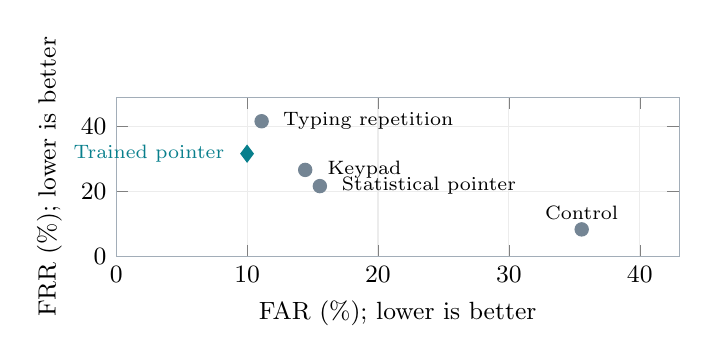
\begin{tikzpicture}
\begin{axis}[width=.72\linewidth,height=36mm,xmin=0,xmax=43,ymin=0,ymax=49,
 xlabel={FAR (\%); lower is better},ylabel={FRR (\%); lower is better},
 tick label style={font=\small},label style={font=\small},grid=major,grid style={gray!15},axis line style={navy!40},clip=false]
\addplot[only marks,mark=*,mark size=2.4pt,color=navy!60] coordinates {(35.56,8.33) (11.11,41.67) (15.56,21.67) (14.44,26.67)};
\addplot[only marks,mark=diamond*,mark size=3pt,color=teal] coordinates {(10,31.67)};
\node[font=\scriptsize,anchor=south] at (axis cs:35.56,8.33){Control};
\node[font=\scriptsize,anchor=west] at (axis cs:12,41.67){Typing repetition};
\node[font=\scriptsize,anchor=west] at (axis cs:16.5,21.67){Statistical pointer};
\node[font=\scriptsize,anchor=west] at (axis cs:15.4,26.67){Keypad};
\node[font=\scriptsize,anchor=east,text=teal] at (axis cs:9,31.67){Trained pointer};
\end{axis}
\end{tikzpicture}
\captionof{figure}{Lower is better on both axes; the preferred direction is toward the lower left. These are conditional policies, not points on a common single-score threshold curve; no app-wide EER is inferred.}
\end{center}

\textbf{Why choose trained pointer?} Its synthetic FAR is lowest (10.00\%); FRR is below typing repetition (31.67\% versus 41.67\%). Against statistical pointer, it prevents five false accepts and adds six net genuine failures. Both challenge 63/150 cases; the encoder decides 33 desktop cases. All 33 scores agree with frozen predictions within 0.000002, and all 300 paired session outcomes were checked. This is a concrete gain for prioritizing unauthorized-access reduction.

\textbf{Is either pointer method statistically superior?} No overall winner is established. An exploratory paired sign-flip test swaps method labels for whole accounts over all $2^{15}$ assignments. Its two-sided FAR/FRR probability values, 0.125/0.156, exceed the conventional 0.05 significance level. They measure extremeness under an exchangeable-method null assumption, not the probability a model is correct. Statistical pointer makes 27 errors versus 28 for trained pointer. On these fixed counts, trained pointer has lower cost when a false accept costs more than 1.2 times a false reject. \emph{Security priorities}, not statistical dominance, motivate the choice.

The nine residual false accepts bypass the encoder: seven owner-like typing attacks and two mobile cases. Across 100 mappings, FAR spans 10.00--13.33\% and FRR 25.00--41.67\%. Fixing an adapter that rejected valid pauses reduces FRR from 50.00\% to 31.67\%. Source-calibration targets 0.1/1/5\% give app FRR 33.33/31.67/28.33\%, with FAR 10\%. The latest mobile timing-rule and threshold changes are functionally tested but postdate these aggregate results.

\section{Conclusion}
BioPrint turns behavioral recognition into an executable strategy: \textbf{recognize familiar behavior efficiently, use device context intelligently, and request a different signal when evidence is insufficient}. Dataset studies establish how nonlinear typing and learned pointer representations improve their baselines; paired studies establish why gains must be transferred selectively. The prototype connects that reasoning to enrollment, model inference and actual access decisions, with a reproducible demonstration of successes and failure modes.

The ablations and paired comparisons make selective integration a defensible design decision: they show which additional evidence helps, its rejection cost, and where generic fusion fails. Trained pointer prevents five additional impostor admissions while preserving direct login for convincing typing. Residual attacks identify the next target: direct-admission verification. This combination of measured improvement, explicit tradeoffs and working integration provides a strong foundation for broader paired-user validation and richer personal models.

\vspace{2pt}\hrule\vspace{3pt}
{\scriptsize\textbf{References and reproducibility.}
[1] NIST, \href{https://pages.nist.gov/800-63-4/sp800-63b.html}{Digital Identity Guidelines: Authentication and Authenticator Management}.
[2] BioCatch, \href{https://www.biocatch.com/what-we-do}{Behavioral biometrics and fraud detection}.
[3] Killourhy and Maxion, \href{https://www.cs.cmu.edu/~keystroke/}{CMU keystroke benchmark}.
[4] scikit-learn, \href{https://scikit-learn.org/1.7/modules/svm.html}{Support Vector Machines}.
[5] Singh et al., \href{https://huggingface.co/datasets/beacon-gui/BEACON-Dataset}{BEACON dataset}.
Experiment tables, source hashes and reproduction instructions accompany the report in the repository.}
\end{document}
